% !TEX root = DesignDocument.tex


\chapter{User Documentation}


%\newpage   %% 
%%  The user guide can be an external document which is included here if necessary ...
%%  a single source is the way to go.

\section{User Guide}
 
 \subsection{Registering a new User}
When you First open the app you will be required to register a user or you can login via Facebook or twitter. To create a Crowd Control account fill out the required page and click register.
 
 \subsection{Login}
 
 \subsubsection{Crowd Control User}
 From the main page click the email button. This will allow you to login in via a Crowd Control account.
 
 
 \subsubsection{Facebook Login}
 From the main page click the Facebook button. This will allow you to login via a Facebook account that will link to a Crowd Control user account.
 
 \subsubsection{Twitter Login}
 From the main page click the twitter button. This will allow you to login via a twitter account that will link to a Crowd Control user account..
 
 \subsection{Creating a Group}
 
 From the main page:
 
 \begin{enumerate}
 \item Click ``CREATE A NEW GROUP'' Button at the bottom of the page.
 \item Fill out Group Name and Group Description
 \item Click ``create group''
 \end{enumerate}
 
 
 \subsection{Joining a Group}
 \subsubsection{From Main List}
 \begin{enumerate}
 \item Find the group from the list that you wish to join.
 \item Click on the group to join.
 \end{enumerate}
 
 \subsubsection{From Invite}
 \begin{enumerate}
 \item Go to notifications.
 \item Click on the invitation to join the group that invited you.
 \end{enumerate}
 
 
 \subsection{Leaving a Group}
 Click the leave group button at the bottom of the main group page.
 
 \subsection{Group Main Page}
 This page shows the main information of the group including:\\
 	\begin{itemize}
 	\item Group Name.
 	\item Description of the Group.
 	\item List of Group Members.
 	\item Leave Button
 	\end{itemize}
 
 
 \subsection{Map Page}
 This page displays a map with pins of the other members in your group
 
 \subsubsection{Sync Map}
 The sync map button will sync the map with the current locations of other members if your group. This feature is for if your map becomes desynced.
 
 \subsubsection{Center Map}
 Clicking on the center map button will center the map on your location.

 \subsection{Messaging Page}
 This is the messaging feature. It allows you to send messages to the rest of the group. To bring up the key board click the text feild at the bottom of the page.
 
 \subsection{Options Menu}
 	\subsubsection{ Notifications}
 		\begin{enumerate}
		\item Opens the notifications page.
 		\end{enumerate}
 	\subsubsection{Settings}
 	\begin{enumerate}
		\item Opens the settings page for CrowdControl.
 	\end{enumerate}
 	
 \subsection{Group Leader Options}

  	\subsubsection{Invite}
  	\begin{enumerate}
		\item Opens the Invite page
 	\end{enumerate}
	\subsubsection{Notifications}
 	\begin{enumerate}
		\item Opens the notifications page.
 	\end{enumerate}
 	\subsubsection{Change Group Name}
 	\begin{enumerate}
		\item Opens a window to change the name of the group
 	\end{enumerate}
 	\subsubsection{Settings}
 	\begin{enumerate}
		\item Opens the settings page for CrowdControl.
 	\end{enumerate}
 
 
 \subsection{Inviting Group Members}
 From the invite page:
 \begin{enumerate}
 \item Select users from the list of users, or you can search for there user name using the search bar.
 \item When you have selected the users you would like to invite click on the next tab for the comfermation screen.
 \item If these are the people you would like to invite click confirm and invites will be sent to the user.
 \end{enumerate}
 
 \subsection{Settings}
 \subsubsection{Changing Profile Name}
 \begin{enumerate}
 \item To change your profile name click the text feild and change the name to the name you wish to be displayed to the rest of the group.
 \item click change name.
 \end{enumerate}
 
 \subsubsection{Search Distance}
 Adjust the search radius for locating a group to join.
 
 \subsubsection{Current Group}
 
 
 \subsubsection{Logout}
 
 \subsubsection{Finished}
 This will bring you back to the home page or the group main page if you are in a group.


%% \newpage  %%  if needed ...
\section{Installation Guide}
\subsection{Android Install}
\subsubsection{AppStore} 
Android Appstore version is not currently avalable.

\subsubsection{Android Studio}

\textbf{Set up your Device}

\begin{enumerate}
\item Plug in your device to your development machine with a USB cable. If you're developing on Windows, you might need to install the appropriate USB driver for your device. 
\item Enable USB debugging on your device. On Android 4.0 and newer, go to Settings > Developer options. 
\end{enumerate}

\textbf{Run the app from Android Studio}\\
\begin{enumerate}
\item Select one of your project's files and click Run from the toolbar.
\item In the Choose Device window that appears, select the Choose a running device radio button, select your device, and click OK .
\end{enumerate}

Android Studio installs the app on your connected device and starts it.\\

Taken from \href{http://developer.android.com/training/basics/firstapp/running-app.html}{http://developer.android.com}.

\subsection{iOS}
\subsubsection{AppStore}

Apple Appstore version is not currently avalable.

\subsubsection{XCode}

\textbf{Launching Your App on a Device}


It takes just a few steps to launch your app on a device if you previously created your code signing identity and team provisioning profile, as described in Creating the Team Provisioning Profile. Otherwise, a series of dialogs and warnings may appear as Xcode resolves the code signing issues in the process of launching your app.\\


\textbf{To launch an app on a device}

\begin{enumerate}
\item Connect the device to your Mac.
\item In the project navigator, choose your device from the Scheme toolbar menu.\\ Xcode assumes you intend to use the selected device for development and automatically registers it for you.\\

	\begin{figure}[tbh]
	\begin{center}
	\fbox{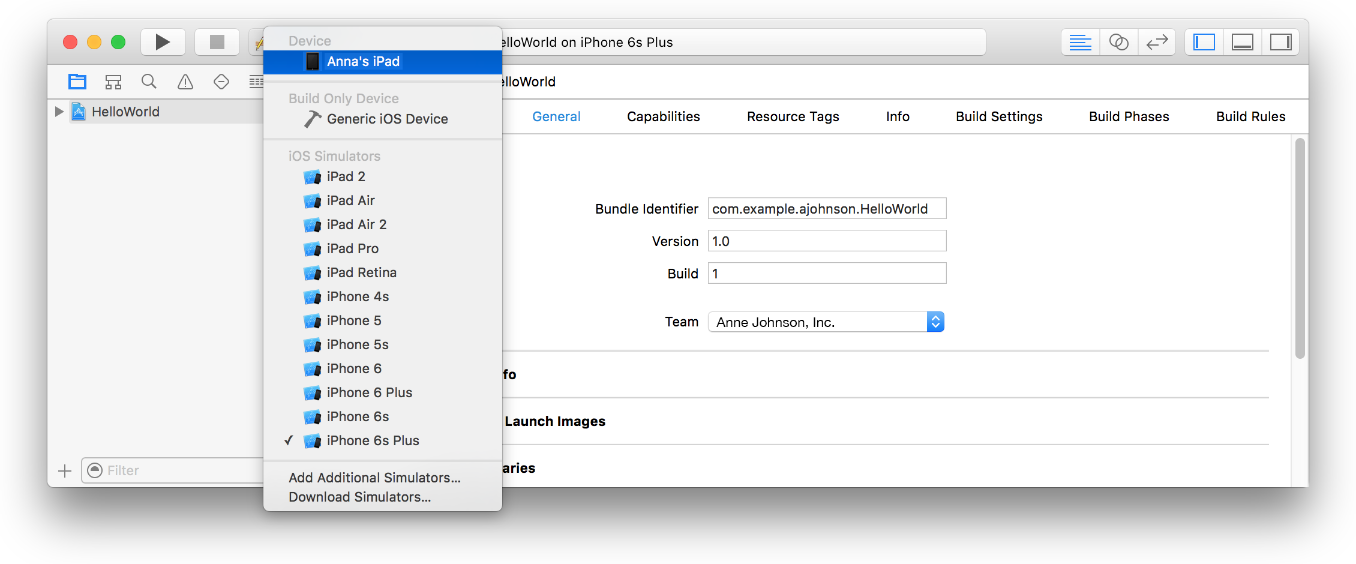
\includegraphics[scale=.4]{Additional/instal/iosAppLaunch.png}}
	\end{center}
	\caption{iOS Device selection \label{iOSDeviceSelection}}
	\end{figure}
	
 If your device is disabled in the Scheme toolbar menu because it is ineligible, fix the issue before continuing. Under Ineligible Devices, hover the mouse over the device to read the reason why it’s ineligible. For example, if the OS version is lower than the deployment target, upgrade the OS version on the device or choose the version you want to target from the Deployment Target pop-up menu (located in the Deployment Info section). Then select the device from the Scheme toolbar menu.
\item If a prompt appears asking whether codesign can sign the app using a key in your keychain, click Always Allow.
\item Click the Run button.\\

Xcode installs the app on the device before launching the app.
\end{enumerate}

Taken from \href{https://developer.apple.com/library/mac/documentation/IDEs/Conceptual/AppDistributionGuide/LaunchingYourApponDevices/LaunchingYourApponDevices.html}{https://developer.apple.com}. 


%% \newpage  %%  if needed ...
\section{Programmer Manual}

\subsection{Api key changes}
The API keys are located in 

	\begin{figure}[tbh]
	\begin{center}
	\fbox{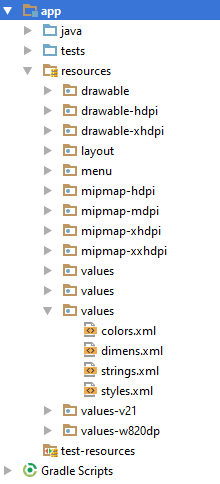
\includegraphics[scale=.4]{Additional/android/apiAndroid.png}}
	\end{center}
	\caption{Android Api Location \label{AndroidApiLocation}}
	\end{figure}
	
	This Is The file where the API keys are held.
	
	\subsection{Global Strings}
	Global strings are located in the same spot that the API keys are located. Theses strings are able to change to implement globalization for expansion to other languages. 
	
	\subsection{Crash handeling}
	Crashalitics is integrated and handles and gives email reports of crashes. Crashalitics will give information such as number of crashes, time, file location and file line.
	
	\subsection{Database} 
	
	Parse handles the database. Values here should not be changed or removed. Tables are able to be added as Crowd Control expands.
